
The CDF collaboration reported evidence~\cite{CDFresult} 
for an excess near 150\GeV in the invariant mass (\mjj) spectrum 
of the two leading-transverse-momentum (\pt) jets
produced in association with a W boson decaying leptonically.  
The D0 collaboration carried out a similar analysis
but could not confirm the result~\cite{D0result}.  
This letter details the search for a similar excess in the \mjj spectrum
using $5.0\fbinv$ of data collected at $\sqrt{s} = 7\TeV$
with the Compact Muon Solenoid (CMS) detector at the CERN 
Large Hadron Collider (LHC) during 2010 and 2011.

Events are selected with one well-identified and isolated lepton,
large missing transverse energy (\met), and two or three high-\pt
jets.  The selection criteria are similar to those used at the
Tevatron~\cite{CDFresult,D0result}, with modifications adapted to the
higher background rates and different experimental conditions at the
LHC.  We also place more stringent requirements on the jet kinematics,
as suggested in~\cite{ELM}, to enhance any signal compared to the
irreducible W+jets background.  We investigate three representative
models, a technicolor $\pi_T$ from the decay of a technicolor
$\rho_T$~\cite{Eichten:2011sh,AMartinMC}, a leptophobic $\zp\to
jj$~\cite{Buckley:2011vc,BuckleyMC}, and the standard model (SM) Higgs
boson produced in association with a W boson (referred to as WH
production) and decaying to jet pairs.

The CMS~\cite{CMSDetector} coordinate system has its origin at the
centre of the detector, with the $z$ axis pointing along the direction
of the anticlockwise beam.  The azimuthal angle is denoted as $\phi$,
the polar angle as $\theta$, and the pseudorapidity is defined as
$\eta = -\ln\tan\left(\theta/2\right)$.

%\section{Event reconstruction and selection}

Jets and \met~\cite{Chatrchyan:2011tn,WZCMS:2010} are reconstructed
from the object collections obtained with the particle-flow
algorithm~\cite{PFT-09-001}, which combines information from several
subdetectors.  Jets are formed with the anti-$k_T$ clustering
algorithm~\cite{ANTIKT} with size parameter 0.5.  We require
$|\eta_{\textrm{jet}}| < 2.4$ to ensure that they lie within the
tracker acceptance.  Charged-particle tracks not originating at the
primary vertex are not considered for jet clustering~\cite{fastjet1,
  fastjet2}.  Jets are required to satisfy identification criteria
that eliminate jets originating from noisy channels in the hadron
calorimeter~\cite{Chatrchyan:2009hy}.  Jet energy
corrections~\cite{Chatrchyan:2011ds} are applied to account for the
jet energy response as a function of $\eta$ and \pt, and to correct
for additional proton-proton interactions occurring within the same
bunch crossing.  The jet \pt resolution varies from 15\% at $\pt =
40\GeV$ to 6\% at $\pt = 400\GeV$~\cite{Chatrchyan:2011ds}.

Electron candidates are identified as clustered energy deposits in the
electromagnetic calorimeter matched to tracks within its coverage,
$|\eta|<1.44$ and $1.57 < |\eta| < 2.5$.  Muon candidates are
reconstructed in the region $|\eta| < 2.1$ by combining information
from the silicon tracker and the muon chambers by means of a global
fit.  Electron and muon candidates need to fulfill quality criteria
established for the measurement of the inclusive W and Z cross
sections~\cite{WZCMS:2010}.  In addition, all leptons must be
well-separated from hadronic activity in the event.  Jets within an
$\eta$-$\phi$ cone of radius 0.3 around a lepton candidate are
removed.

The data were collected with a suite of single-lepton triggers, mostly
with a \pt requirement of 24\GeV for muons and 25--32\GeV for
electrons.  The selection criteria are listed in
Table~\ref{tab:SELECTION}.  The trigger efficiency for the selected
muons (electrons) is about 94\% (90\%).  The transverse mass $\MT$ of
a W candidate is defined as $\MT \equiv {\small
  \sqrt{2\pt^\ell\,\met\,[1-\cos(\phi_\ell-\phi_{\met})]}}$, where
$\phi_\ell$ and $\phi_{\met}$ are the azimuthal angles of the lepton
and $\met$, respectively.  The selected jets and the lepton from the
W decay are required to originate from the same primary vertex.
The requirement $0.3 < \pt^{\text{2nd~jet}}/\mjj < 0.7$ is imposed to
take advantage of the separation in this variable between resonant
dijet production when compared to nonresonant W+jets production.

\begin{table}[tb]
\caption{\label{tab:SELECTION}Selection criteria summary.}
\begin{ruledtabular}
\begin{tabular}{ll}
  \Wln\ selection  & Jet selection \\
  \hline 
  single-lepton trigger &   $\pt^{\text{lead~jet}} > 40\GeV$ \\
  tight identification and isolation & $\pt^{2^\text{nd} \text{~or~} 3^\text{rd} \text{~jet}} > 30\GeV$ \\
  $\pt^{\mu (\Pe)}> 25~(35)\GeV$ & dijet $\pt > 45\GeV$  \\
  $\met^{\hspace{0.8mm}\mu (\Pe)} > 25~(30)\GeV$ & $|\Delta \eta_{jj}| \le 1.2$ \\
  $\MT > 50\GeV$ & $\Delta \phi (\met,\text{lead~jet}) > 0.4$ \\
  second lepton veto & $0.3 < \pt^{\text{2nd~jet}}/\mjj < 0.7$
\end{tabular}
\end{ruledtabular}
\end{table}

%\section{Data and simulated event samples}
The selected sample is dominated by events containing a W plus
two or more jets.  
Smaller contributions come from top-pair and single-top decays, 
Drell--Yan plus two or more jets, and multijet production.
A small fraction of events is due to WW and WZ diboson 
production with one W decaying leptonically and the other 
W or Z decaying hadronically.  

Large samples of simulated events of various SM processes are used to
model the shapes of their \mjj distributions.  The
\MADGRAPH~\cite{MADGRAPH} event generator produces parton-level events
with a W boson and up to four partons on the basis of
matrix-element (ME) calculations.  The ME--parton shower matching
scale $\mu$ is taken to be 20\GeV and the factorization and
renormalization scales are set to $q^2 = M_{W}^2 +
p_{\mathrm{T},W}^2$.  Four additional samples of W events are
generated with the scales increased and reduced by a factor of two
with respect to those of the reference sample.  Samples of \ttbar\ and
Drell--Yan events are also generated with \MADGRAPH.  Single-top
production is modelled with {\sc powheg}~\cite{POWHEG}.  Multijet and
diboson samples (WW, WZ, ZZ) are generated with
\PYTHIA~\cite{Sjostrand:2006za}.  \PYTHIA provides the parton shower
simulation in all cases, with parameters of the underlying event set
to the Z2 tune~\cite{PythiaTuneZ2}.  The set of parton distribution
functions used is CTEQ6LL~\cite{CTEQ}.  Simulated signal samples for
the technicolor and WH models are generated with \PYTHIA, while the
leptophobic $\zp$ is generated with \MADGRAPH.  A GEANT4-based
simulation~\cite{GEANT4} of the CMS detector is used in the production
of all Monte Carlo (MC) samples.  Multiple proton-proton interactions
within a bunch crossing are taken into account, and the triggers are
emulated.  All simulated events are reconstructed and analyzed with
the same software as collision data.  We correct for any differences
in the performance of the trigger, lepton reconstruction, and $\met$
resolution between data and simulation.

We determine the relative contributions of the known SM processes to
the observed \mjj spectrum by means of an unbinned maximum-likelihood
fit in the range between 40\GeV and 400\GeV.  The fit is performed
separately for the electron and muon channels and for the 2-jet and
3-jet samples because the background compositions differ.  The
\mjj signal region, 123 to 186\GeV, which corresponds to about a
${\pm} 2\sigma$ window, is excluded from this fit in order to arrive
at an unbiased estimate of a possible resonant enhancement in this
region.

\begin{table}[bt]
 \caption{Determination of the shapes and normalizations of the \mjj distributions. 
 External constraints are assumed to be Gaussian.}  
 \label{tab:Table0} 
\begin{ruledtabular}
\begin{tabular} {lcl}
   Process             &    Shape     & Constraint on normalization \\ 
   \hline
   W+jets              &    MC/data   & Unconstrained \\
   Diboson             &    MC        & (NLO) 61.2 pb $\pm 10\%$~\cite{Campbell:2011bn}\\ 
   \ttbar\             &    MC        & (NLO) 163 pb $\pm 7\%$~\cite{Kidonakis:2010dk}\\ 
   Single-top          &    MC        & (NNLO) $\pm 5\%$~\cite{Kidonakis:2010tc,Kidonakis:2011wy,Kidonakis:2010ux}\\
   Drell--Yan + jets   &    MC        & (NNLO) 3.05 nb $\pm 4.3\%$~\cite{FEWZ} \\
   Multijet            &    data      & \met fit (described in text) \\
 \end{tabular}
\end{ruledtabular}
\end{table}

Table~\ref{tab:Table0} lists the SM processes included in the fit.
The normalization of the dominant W+jets contribution is a free fit
parameter.  The normalizations of the other background components are
allowed to vary within Gaussian constraints around their central
values.  For multijet events, this central value is obtained from a
separate fit to the $\met$ distribution~\cite{WZCMS:2010}, and the
constraint is driven by the corresponding fit error estimate.  The
central values for all other processes are obtained from
next-to-leading-order (NLO) or next-to-NLO (NNLO) calculations, and
the constraints reflects the theoretical uncertainties.  With the
exception of multijet production, the \mjj distribution shapes for all
processes are obtained from simulation.  Multijet events contribute
when jets are misidentified as isolated leptons; the shape of the \mjj
distribution for multijet events can therefore be derived from data
events with lepton candidates that fail the isolation requirements.

The \mjj spectrum of the dominant W+jets component is not well
described by \MADGRAPH.  No significant improvement is observed with
the alternative samples.  We employ a combination of three shapes to
describe this component in the fitting function:
\begin{linenomath}
\begin{align}
F_{\text{W+jets}} = \alpha\, & \mathcal{F}_{\text{W+jets}} (\mu_{0}^2, q'^2) + 
\beta\, \mathcal{F}_{\text{W+jets}} (\mu'^2, q_{0}^2) \nonumber \\ 
&+ (1-\alpha-\beta)\, \mathcal{F}_{\text{W+jets}} (\mu_{0}^2, q_{0}^2)\,,
\label{eqWpjetsShape}
\nonumber
\end{align}
\end{linenomath}
where $\mathcal{F}_{\text{W+jets}}$ denotes the \mjj shape from
simulation.  The parameters $\mu_0$ ($\mu'$) and $q_0$ ($q'$)
correspond to the default (alternative) values of $\mu$ and $q$,
respectively, and fractional contributions $\alpha$ and $\beta$ are
free to vary in the fit.  We take $\mu' = 2 \mu_0$ if $\beta>0$ and
$\mu' = 0.5 \mu_0$ if $\beta<0$; similarly, $q' = 2 q_0$ if $\alpha>0$
and $q' = 0.5 q_0$ if $\alpha<0$.

\begin{figure*}[tbh]
  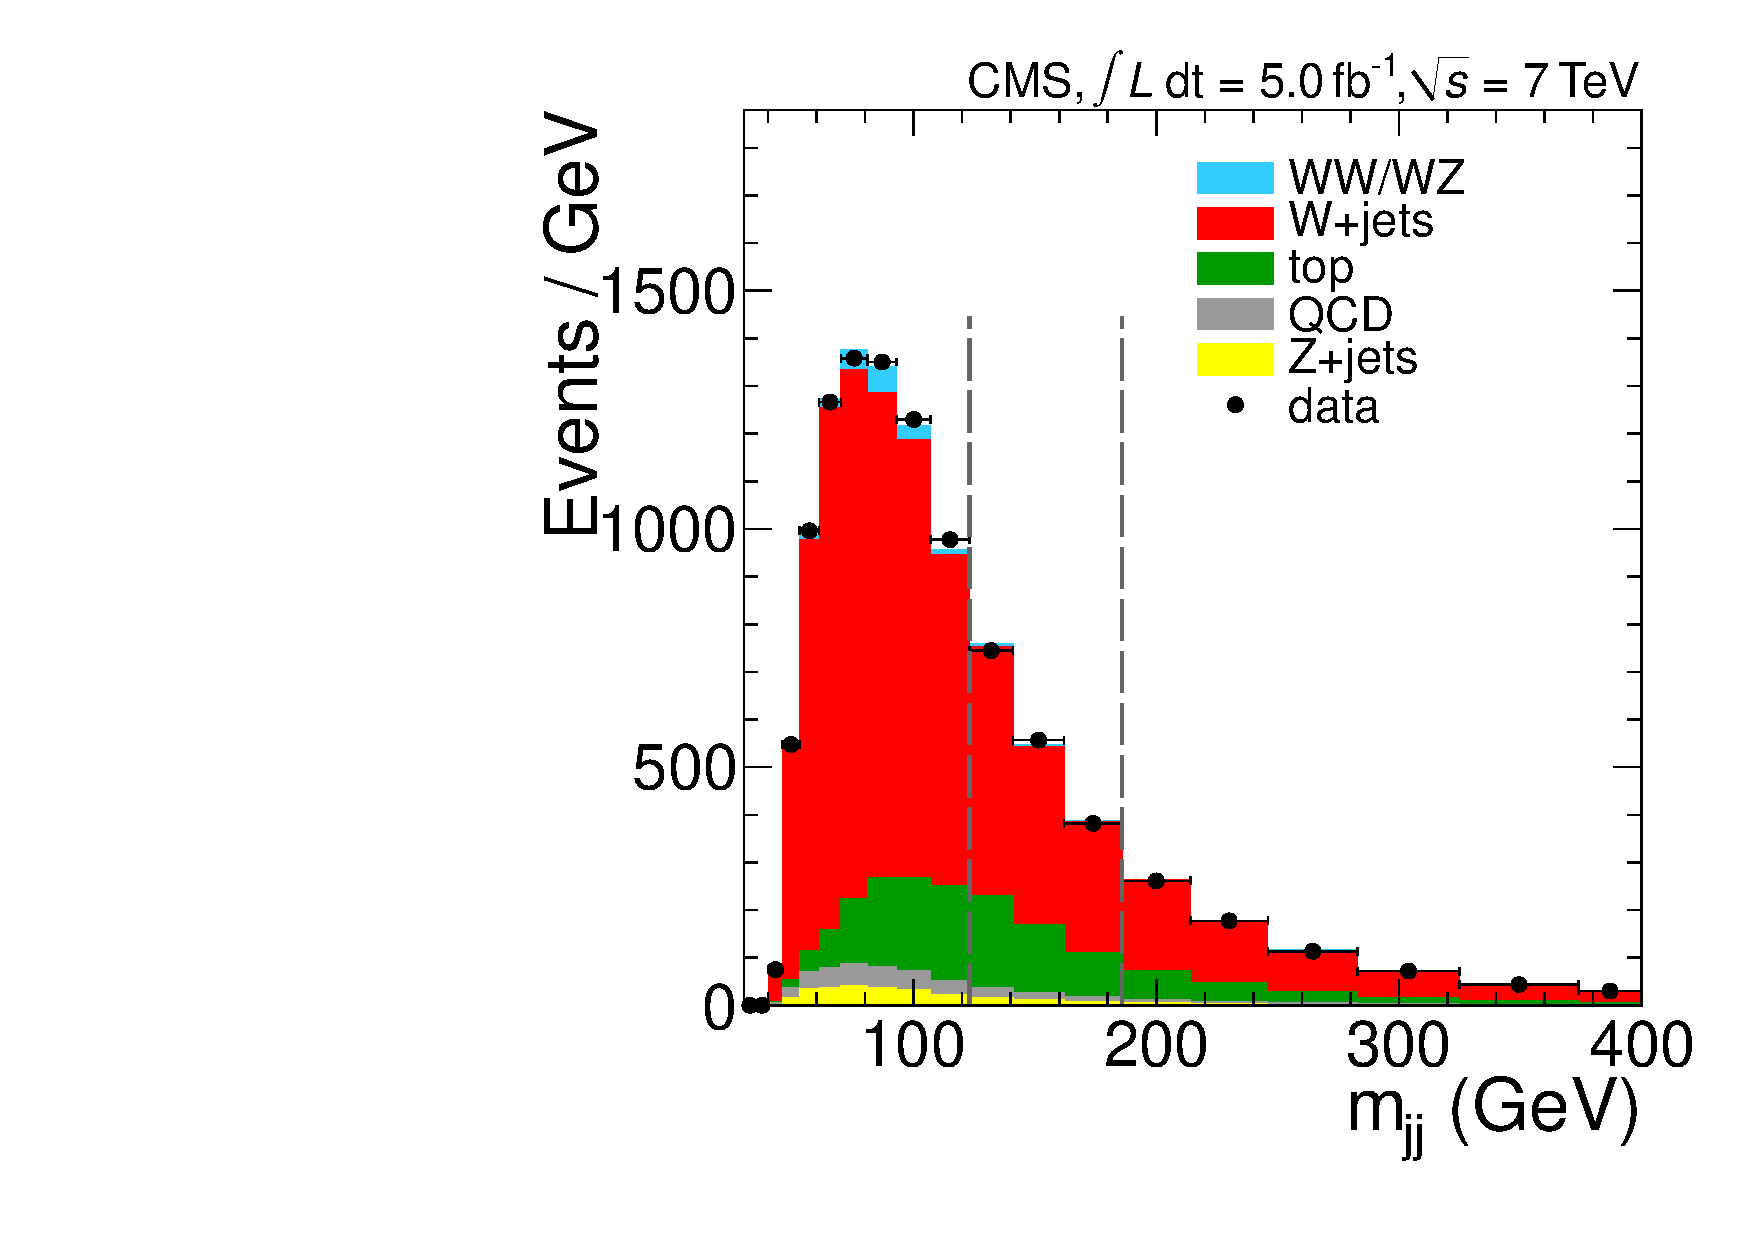
\includegraphics[width=0.32\textwidth]{figs/Mjj_Stacked_combined.pdf}
  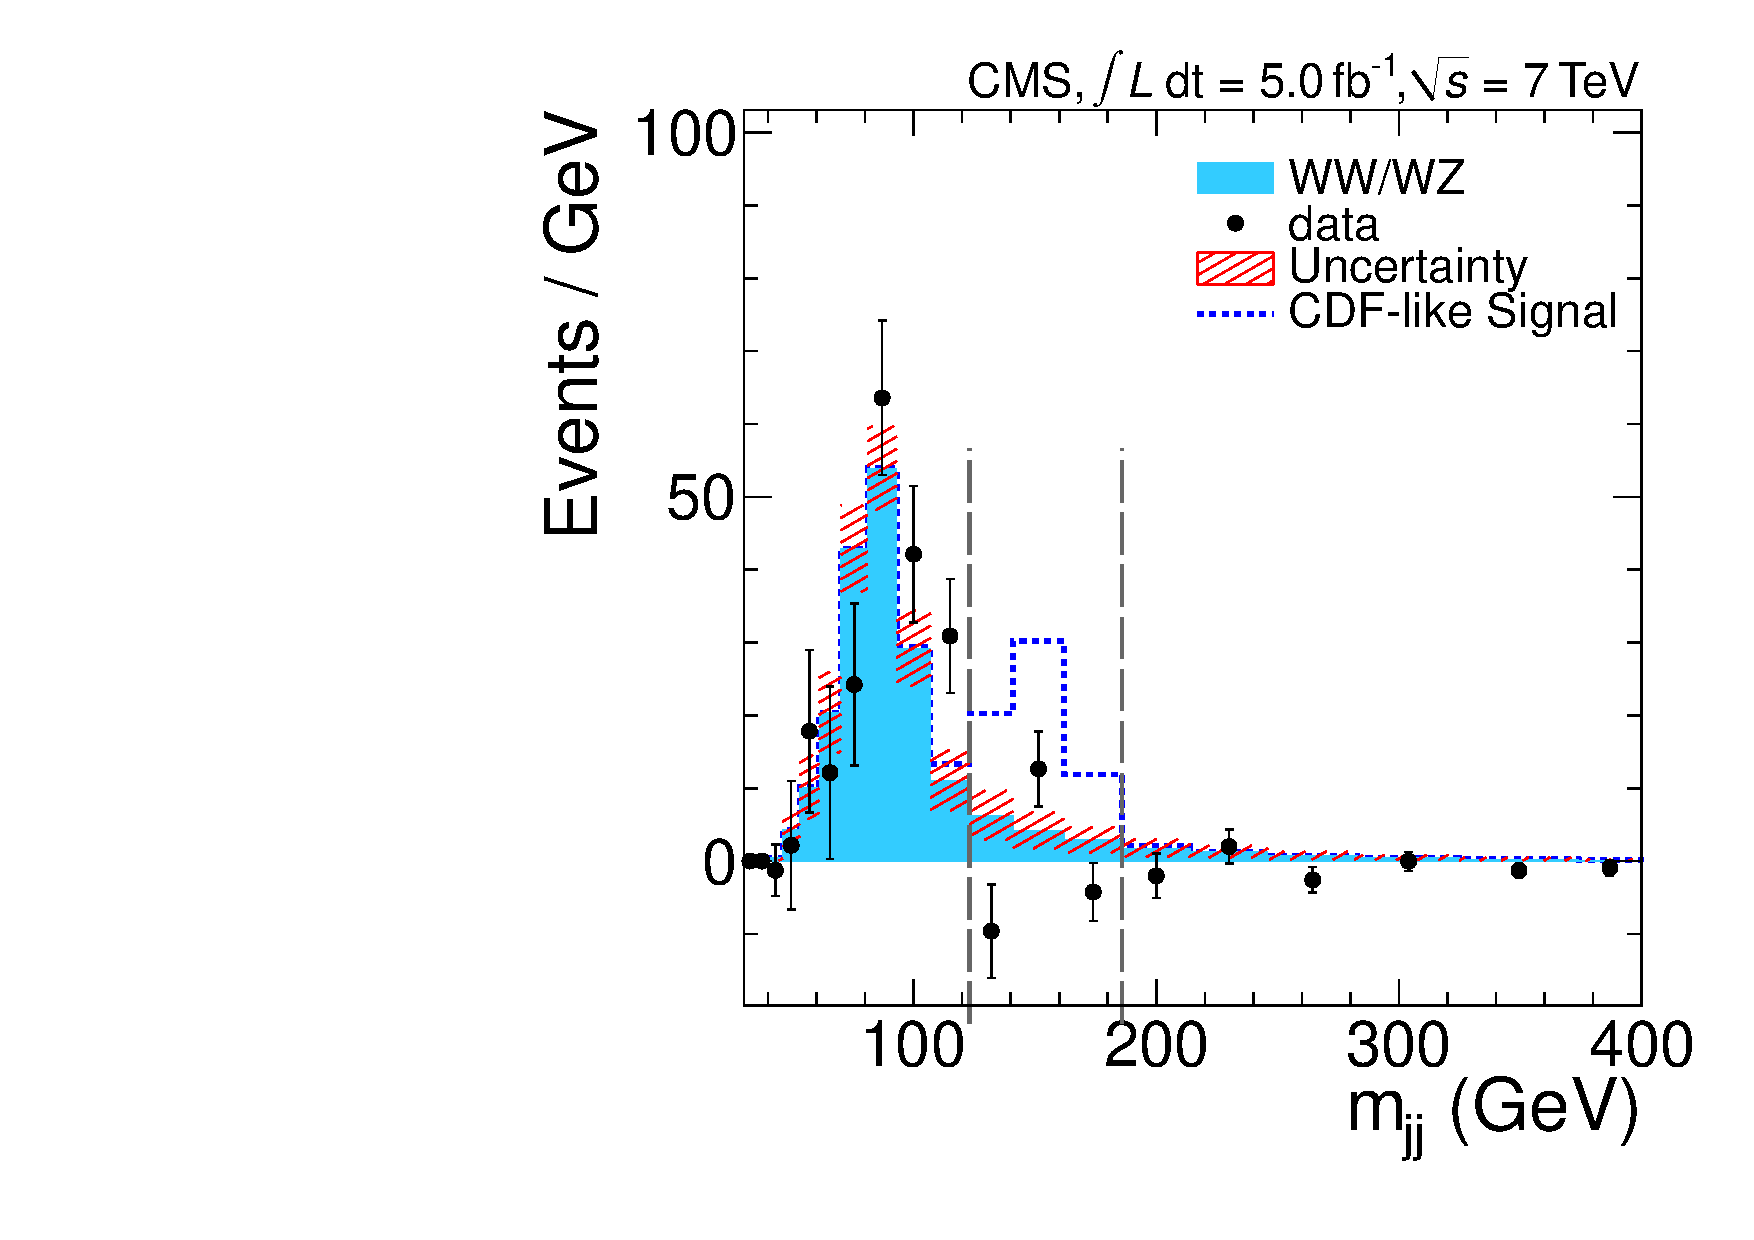
\includegraphics[width=0.32\textwidth]{figs/Mjj_Subtracted_combined.pdf}
  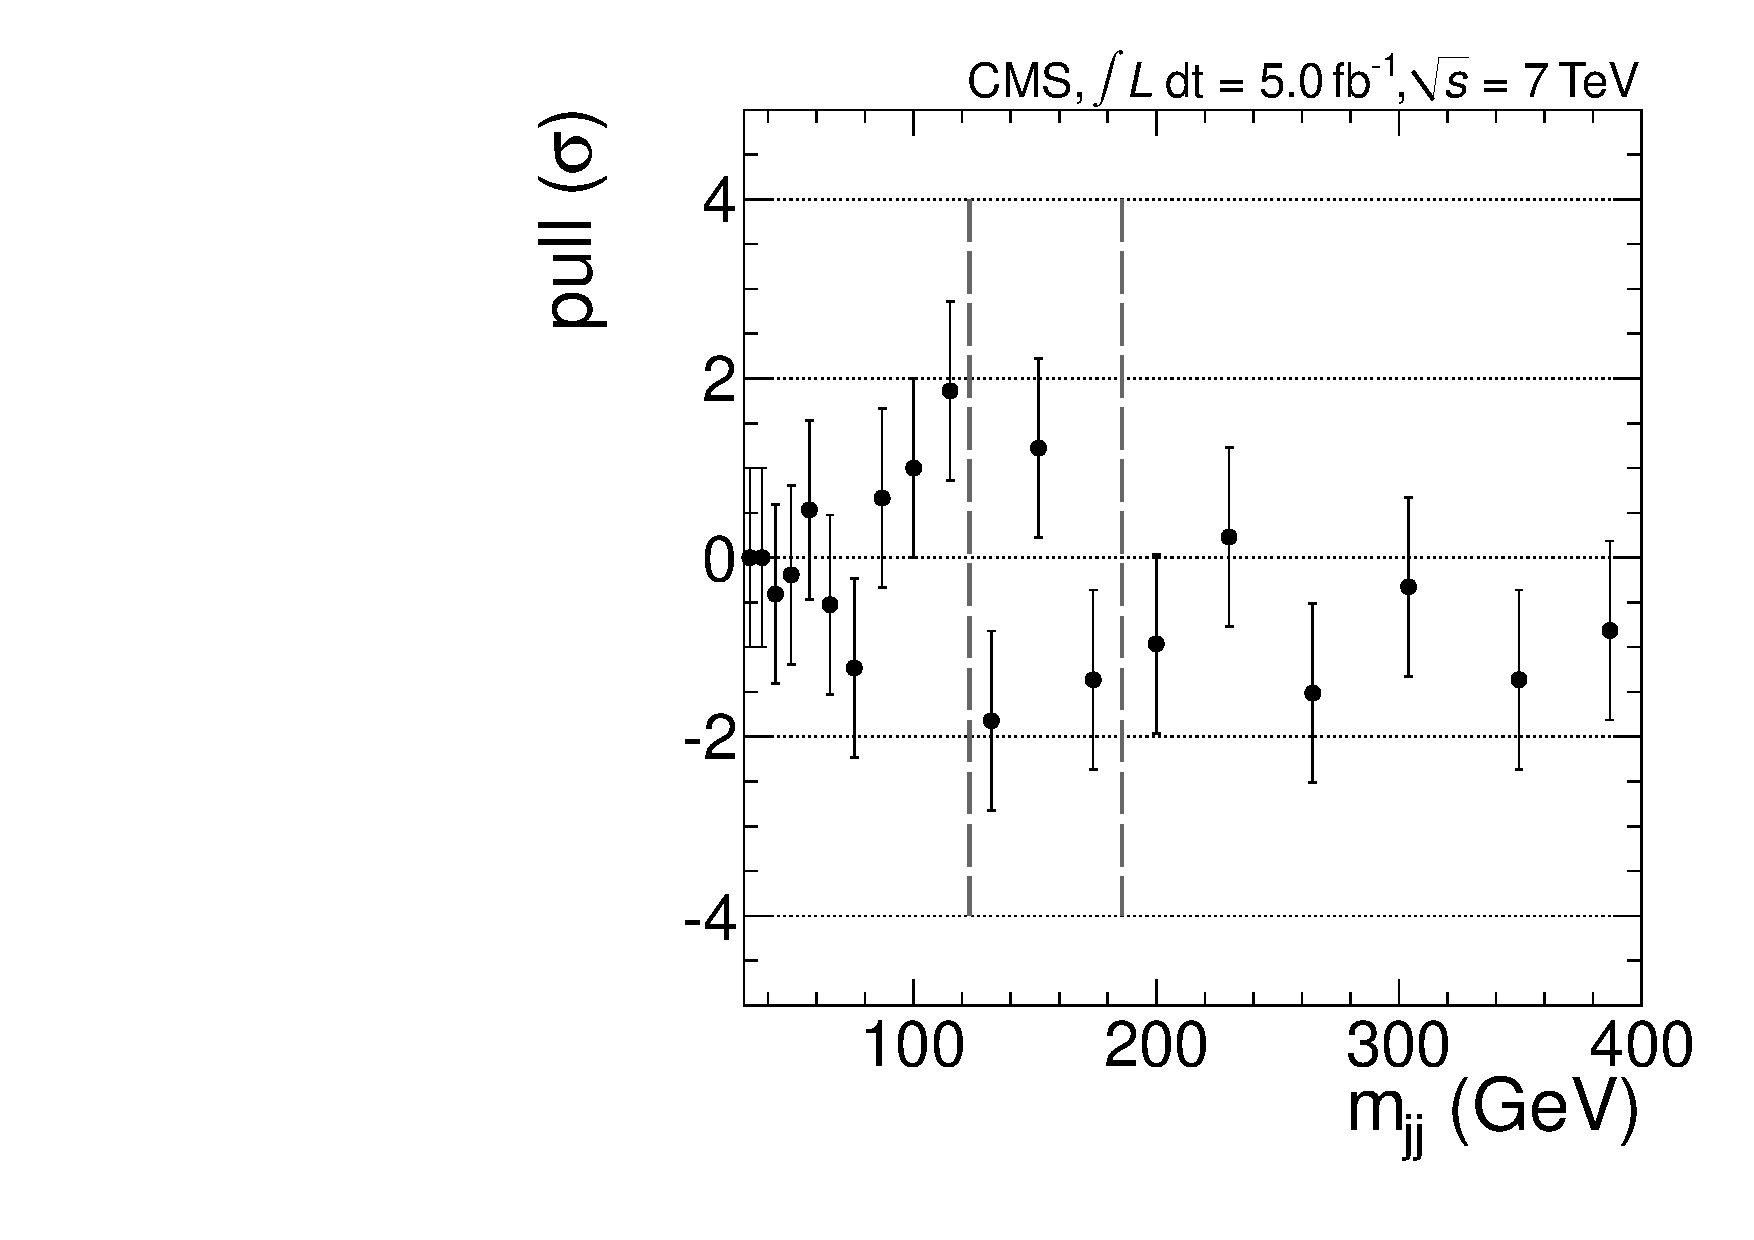
\includegraphics[width=0.32\textwidth]{figs/Mjj_Pull_combined.pdf}
  \caption{(a) Distribution of the invariant mass spectrum of the
    leading two jets observed in data. Overlaid are the fit
    projections of the various components.  The region between the
    vertical dashed lines is excluded from the fit.  Depicted is the
    number of events per GeV, i.e.\ the raw event count can
    be obtained by multiplying with the bin width.  (b)~The same
    distribution after subtraction of all SM components except the
    electroweak diboson WW/WZ.  Error bars correspond to the
    statistical uncertainties.  The band represents the systematic
    uncertainty on the sum of the SM components.  (c)~The normalized
    residual, $(\text{data} - \text{fit})/\text{fit uncertainty}$.}
    \label{fig:Fig1}
\end{figure*}

\begin{table*}[htbp]
  \caption{Event yields determined from a maximum-likelihood fit to the data. 
  The total uncertainty includes the effect of correlation among the 
  individual contributions using the full covariance matrix.}
  \label{tab:yields}
\begin{ruledtabular}
  \begin{tabular} {lcccc}
                        & \multicolumn{2}{c}{Muon channel}  & \multicolumn{2}{c}{Electron channel} \\
   Process              & 2-jet         & 3-jet       & 2-jet          & 3-jet \\
\hline
   W+jets               & $58919 \pm 530$ & $13069 \pm 366$ & $29787 \pm 1153$ & $8397 \pm 292$ \\
   Dibosons             & $1236 \pm 114$  & $333 \pm 32$    & $685 \pm 65$     & $184 \pm 18$ \\
   \ttbar               & $4570 \pm 307$  & $9049 \pm 382$  & $2556 \pm 174$   & $4265 \pm 253$ \\
   Single top           & $1765 \pm 87$   & $1001 \pm 50$   & $916 \pm 46$     & $521 \pm 26$ \\
   Drell--Yan plus jets & $1837 \pm 79$   & $561 \pm 24$    & $1061 \pm 46$    & $364 \pm 16$ \\
   Multijet (QCD)       & $29 \pm 284$    & $0 \pm 90$      & $3944 \pm 1133$  & $324 \pm 160$ \\
\hline
%  Fit $\chi^2$ probability&   0.454      & 0.729           & 0.969            & 0.991 \\
   Total from fit       & $68294 \pm 307$ & $24013 \pm 193$ & $38949 \pm 228$  & $14055 \pm 143$ \\
   Data                 & 67900           & 24046           & 38973            & 14145 \\
\hline
\multicolumn{5}{c}{In the test region $123 < m_{jj} < 186\GeV$ excluded from the fit} \\
\hline
   Total                & $14511 \pm 125$ & $7739 \pm 95$   & $7944 \pm 92$    & $4347 \pm 70$ \\
   Data                 & 14050           & 7751            & 8023             & 4438 \\
  \end{tabular}
\end{ruledtabular}
\end{table*}

Figure~\ref{fig:Fig1}(a) shows the observed \mjj distribution for all
four channels combined, together with the fitted projections of the
contributions of various SM processes.  Figure~\ref{fig:Fig1}(b) shows
the same distribution after subtraction of all SM contributions from 
data except electroweak diboson WW/WZ events.  No peak is visible in
the spectrum except that near 80\GeV due to diboson events.
Figure~\ref{fig:Fig1}(c) shows the normalized residual, i.e.\ the pull
distribution defined as $(\text{data} -
\text{fit})/\text{fit uncertainty}$.  Table~\ref{tab:yields} presents the
yields of various SM components obtained from the fit.  The sum of all
the contributions is compared with the number of observed data events.
All numbers but those in the last two rows are for the \mjj range of
40 to 400\GeV.  The last two rows compare the observed and fitted
contributions in the \mjj range of 123 to 186\GeV, which we exclude
from the fit.  The data agree with the SM expectations, and we find no
significant excess in the test region.

%\section{Fit validation and systematic error estimate}

We validate the fit procedure by performing pseudo-experiments.  In
each experiment, we generate the \mjj pseudo-data of the SM processes,
taking into account the correlation among the yields, and then fit
each pseudo-data sample.  The results indicate that the bias on the
total yield is below 0.2\% and that the fit underestimates the yield
uncertainty slightly.  These effects are corrected for in the final
result.  Uncertainties in the jet energy are estimated in a sample of
W bosons decaying hadronically in a pure sample of semileptonic
\ttbar\ events.  The mean and resolution of the reconstructed dijet
(i.e.,\ W) mass distribution in data agree within 0.6\% with the
expectation from simulation.  A small difference in \met
resolution~\cite{Chatrchyan:2011tn} between data and simulation
affects the signal acceptance for the new physics models under
consideration at the 0.5\% level.  Further systematic uncertainties
are due to the uncertainty of the trigger efficiency estimates in data
(1\%), and the estimate of lepton reconstruction and selection
efficiency (2\%)~\cite{WZCMS:2010}.  The uncertainty on the integrated
luminosity is 2.2\%~\cite{lumiPAS}.
 
%\section{Results on presence of possible resonant enhancement}

We scrutinize the dijet mass spectrum near 150\GeV, searching for a
technicolor, leptophobic $\zp$, or WH resonant enhancement.  We also
use a generic Gaussian signal model obtained from a delta function at
$\mjj=150\GeV$ convolved with the CMS detector resolution of 15\GeV.
The expected number of signal events at the LHC, $N^{\text{signal}}$,
for a given cross section at the Tevatron can be estimated by
considering the ratio of the predicted cross sections for our
reference process, WH production with $M_{\text{H}} = 150\GeV$.  This 
process is dominated by quark-antiquark (\cPq\cPaq) annihilation.  As
\cPq\cPaq\ processes have the smallest increase in partonic luminosity
from the Tevatron to the LHC, this choice provides a conservative
limit.  We therefore assume
\begin{linenomath}
\begin{equation}
\sigma_{\text{LHC}}^{\text{dijet resonance}} = 
\sigma_{\text{Tevatron}}^{\text{dijet resonance}}  
\frac{\sigma_{\text{LHC}}^{WH}}{\sigma_{\text{Tevatron}}^{WH}},\label{eqTevToLHC2}\nonumber
\end{equation}
\end{linenomath}
where $\sigma_{\text{LHC}}^{WH} = 300.1\unit{fb}$~\cite{LHC4PDFxsec}
and $\sigma_{\text{Tevatron}}^{WH} = 71.8\unit{fb}$~\cite{Carena:2000yx}.
The expected yield is then
\begin{linenomath}
\begin{equation}
N^{\text{signal}} = \sigma_{\text{LHC}}^{\text{dijet resonance}} \cdot 
\mathcal{B}(\text{W}\to\ell\nu) 
\cdot (\varepsilon\mathcal{A}) 
\cdot \int \mathcal{L}\ \text{d}t, 
\label{eqTevToLHC}
\nonumber
\end{equation}
\end{linenomath}
where $\varepsilon\mathcal{A}$ denotes $\text{efficiency} \times
\text{acceptance}$ for WH events, $\mathcal{B}(\text{W}\to\ell\nu) = 0.2132
\pm 0.0020$~\cite{pdg} (summing $e$ and $\mu$), and $\int \mathcal{L}
\text{dt} = 5.0\,\text{fb}^{-1}$ is the integrated luminosity.

The values of cross section and $\varepsilon\mathcal{A}$ 
for the models considered are given in Table~\ref{tab:signals}.  
A generic Gaussian signal normalized to
$\sigma_{\text{Tevatron}} = 4\unit{pb}$ corresponds to
$\sigma_{\text{LHC}}\times \mathcal{B}(\text{W}\to\ell\nu) = 3.6\unit{pb}$.
%%%%%%%%%%%%%%%%%%%%%%%
\begin{table}[bt]
  \caption{\label{tab:signals}
    The cross section times $\text{W}\to\ell\nu$ branching fraction 
    and overall efficiency for various signal models.  For the WH model the
    Higgs boson decays generically.}
\begin{ruledtabular}
  \begin{tabular}{l c c c c c}
    &   & \multicolumn{4}{c}{$\varepsilon\mathcal{A}$} \\
    &   & \multicolumn{2}{c}{$\mu$ channel} & \multicolumn{2}{c}{\Pe\ channel} \\
    Signal model &  $\sigma\times\mathcal{B}$ (pb) & 2-jet & 3-jet & 2-jet & 3-jet \\
    \hline
    WH~\cite{Sjostrand:2006za}                  & 0.0145 & 0.060 & 0.019 & 0.038 & 0.013 \\
    Technicolor~\cite{Eichten:2011sh,AMartinMC} & 1.58   & 0.065 & 0.020 & 0.039 & 0.011 \\
    $\zp$~\cite{Buckley:2011vc,BuckleyMC}       & 1.72   & 0.070 & 0.023 & 0.042 & 0.014 \\
  \end{tabular}
\end{ruledtabular}
\end{table}
%%%%%%%%%%%%%%%%%%%%%%%
\begin{figure}[bt]
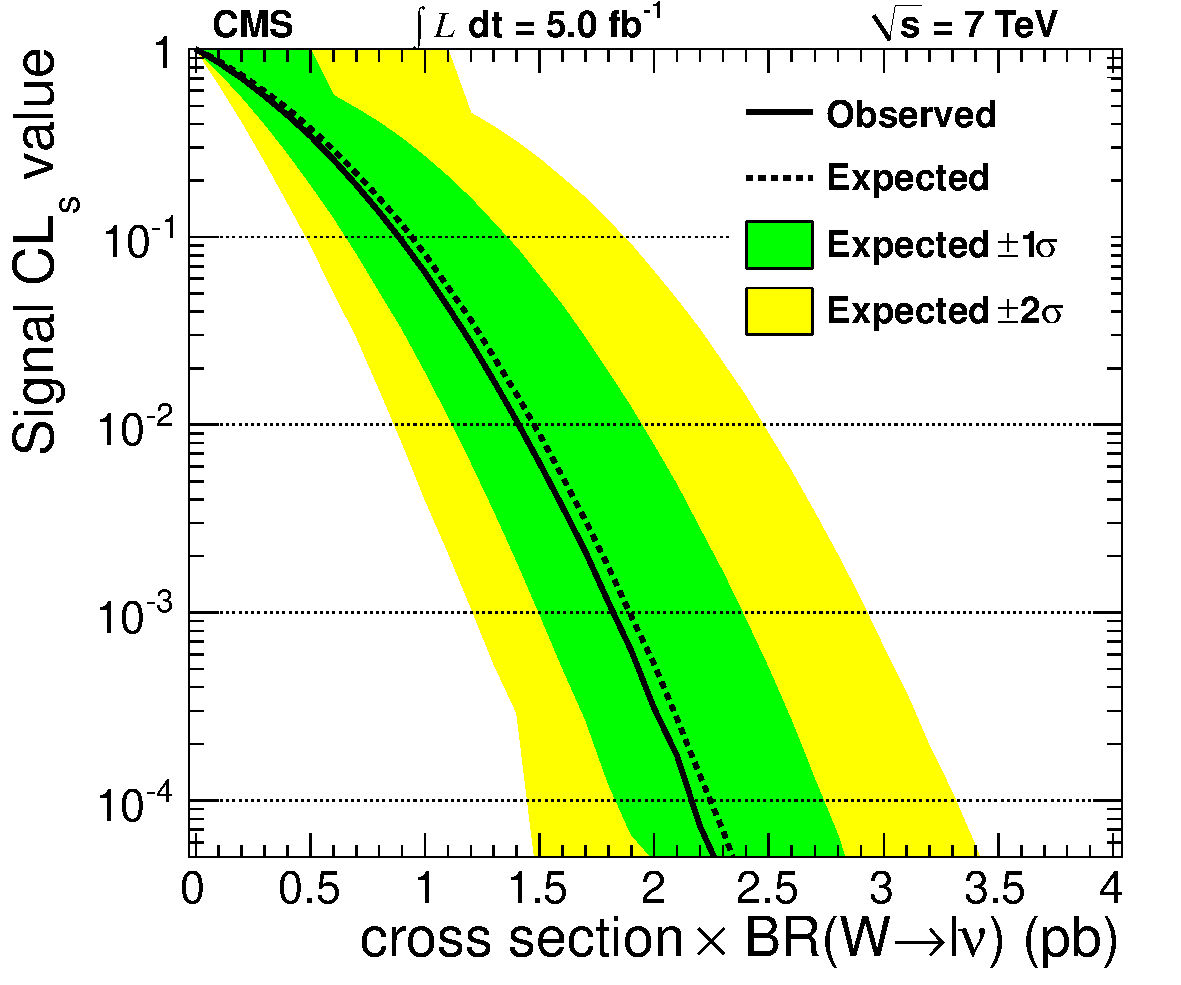
\includegraphics[width=0.4\textwidth]{figs/mjjpvalues.pdf}
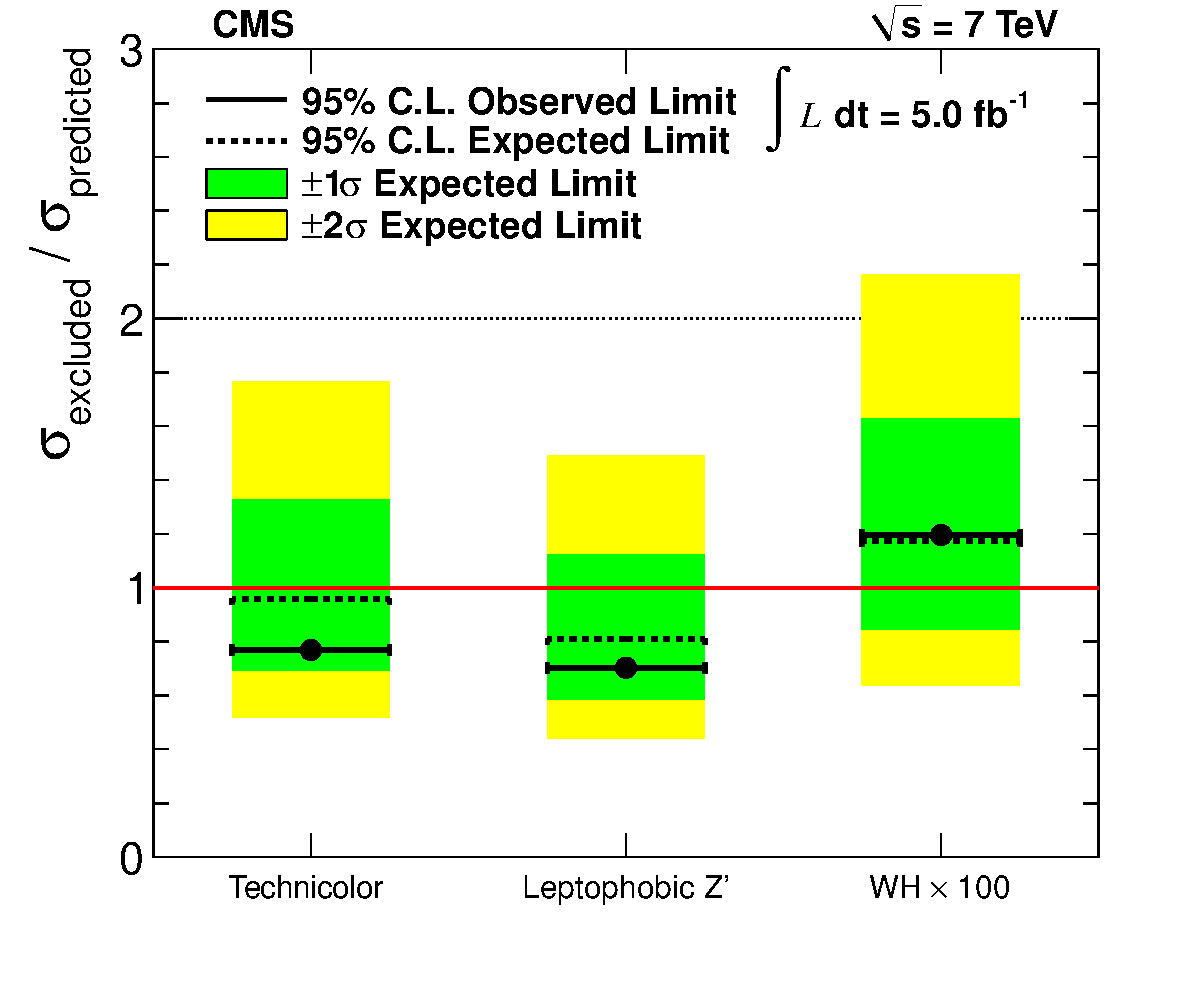
\includegraphics[width=0.4\textwidth]{figs/mjjlimitbars.pdf}
\caption{\label{fig:Fig2}(a) The observed and expected values of the
  $\text{CL}_{\text{S}}$ statistic for a generic Gaussian signal
  hypothesis with $M=150\GeV$ and $\sigma=15\GeV$, as a function of the 
  signal cross section times the $\text{W}\to\ell\nu$ branching fraction.
  (b)~Observed and expected 95\% CL upper limits, with one- and two-sigma 
  error bands, on the cross section divided by the expected values
  for various signal models. 
  The limits are calculated using the $\text{CL}_{\text{S}}$
  method. A value of the excluded cross section over the predicted
  cross section of less than one indicates that the model is excluded
  at 95\% CL.  Table~\ref{tab:signals} lists the cross sections for
  these models.  }
\end{figure}
%%%%%%%%%%%%%%%%%%%

%\vspace{10mm}\noindent
%{\large Language editing ends here\ldots}
%\vspace{10mm}

Since we observe no resonant enhancement, we proceed to set exclusion
limits using a modified frequentist
$\text{CL}_{\text{S}}$ method~\cite{pdg,CLS} with profile likelihood as the
test statistic.  Inputs to the limit-setting procedure are the \mjj
distribution obtained by combining the SM components from the fit, the
observed distribution in data, and the expectation from the dijet
resonance model under consideration.  Figure~\ref{fig:Fig2}(a) shows the
observed and expected $\text{CL}_{\text{S}}$ values
versus cross section times $\mathcal{B}(\text{W}\to\ell\nu)$
for a generic Gaussian signal, after combining the results of all four
event categories.
We set a 95\% confidence level (CL) upper limit of 1.1\unit{pb} on the
production cross section times $\mathcal{B}(\text{W}\to\ell\nu)$ 
for a generic resonance;
the value of $\varepsilon\mathcal{A}$ from the WH process
is used to calculate the limit for the generic signal.

Figure~\ref{fig:Fig2}(b) compares the 95\% CL upper limits with the
expected cross sections for 
technicolor, leptophobic $\zp$, and WH ($M_{\text{H}} = 150\GeV$) signals.
The technicolor and $\zp$ models are excluded, 
but we have minimal sensitivity to WH and compare the limit to
100 times the SM cross section for illustration.

In summary, we have studied the invariant mass spectrum of the
two jets with highest transverse momentum in 
$\text{pp}\rightarrow \text{W+2-jet}$
and W+3-jet events,
with the W decaying leptonically.
The analyzed data sample corresponds to an integrated
luminosity of 5.0\fbinv at $\sqrt{s} = 7\TeV$
collected in 2010 and 2011 with the CMS detector.
We find no evidence for a resonant enhancement near a dijet mass of 150\GeV.  
Several theoretical models that predict the presence of a 
resonant enhancement near 150\GeV are excluded.

% >> acknowledgements (for journal papers)
% Please include the latest version from https://twiki.cern.ch/twiki/bin/viewauth/CMS/Internal/PubAcknow.
%\section*{Acknowledgements}

We congratulate our colleagues in the CERN accelerator departments for
the excellent performance of the LHC machine. We thank the technical
and administrative staff at CERN and other CMS institutes, and
acknowledge support from: FMSR (Austria); FNRS and FWO (Belgium);
CNPq, CAPES, FAPERJ, and FAPESP (Brazil); MES (Bulgaria); CERN; CAS,
MoST, and NSFC (China); COLCIENCIAS (Colombia); MSES (Croatia); RPF
(Cyprus); MoER, SF0690030s09 and ERDF (Estonia); Academy of Finland,
MEC, and HIP (Finland); CEA and CNRS/IN2P3 (France); BMBF, DFG, and
HGF (Germany); GSRT (Greece); OTKA and NKTH (Hungary); DAE and DST
(India); IPM (Iran); SFI (Ireland); INFN (Italy); NRF and WCU (Korea);
LAS (Lithuania); CINVESTAV, CONACYT, SEP, and UASLP-FAI (Mexico); MSI
(New Zealand); PAEC (Pakistan); MSHE and NSC (Poland); FCT (Portugal);
JINR (Armenia, Belarus, Georgia, Ukraine, Uzbekistan); MON, RosAtom,
RAS and RFBR (Russia); MSTD (Serbia); MICINN and CPAN (Spain); Swiss
Funding Agencies (Switzerland); NSC (Taipei); TUBITAK and TAEK
(Turkey); STFC (United Kingdom); DOE and NSF (USA).

